\documentclass[12pt,a4paper]{article}
\usepackage{geometry}
\geometry{left=2.5cm,right=2.5cm,top=2.0cm,bottom=2.5cm}
\usepackage[english]{babel}
\usepackage{amsmath,amsthm}
\usepackage{amsfonts}
\usepackage[longend,ruled,linesnumbered]{algorithm2e}
\usepackage{fancyhdr}
\usepackage{ctex}
\usepackage{array}
\usepackage{listings}
\usepackage{color}
\usepackage{graphicx}
\usepackage{float}
\usepackage{caption}
\begin{document}
    \title{\heiti{《机器学习》课程第 {$1$} 次作业}}
    \date{}
    \author{姓名:\underline{刘哲}~~~~~~学号:\underline{2022103691}~~~~~~}
    \maketitle
    \section{\heiti{生鲜销量}}
    \vspace{10pt}
    \subsubsection*{A}
    生鲜销量数据的时间序列图如下:
    \begin{figure}[H]
        \centering
        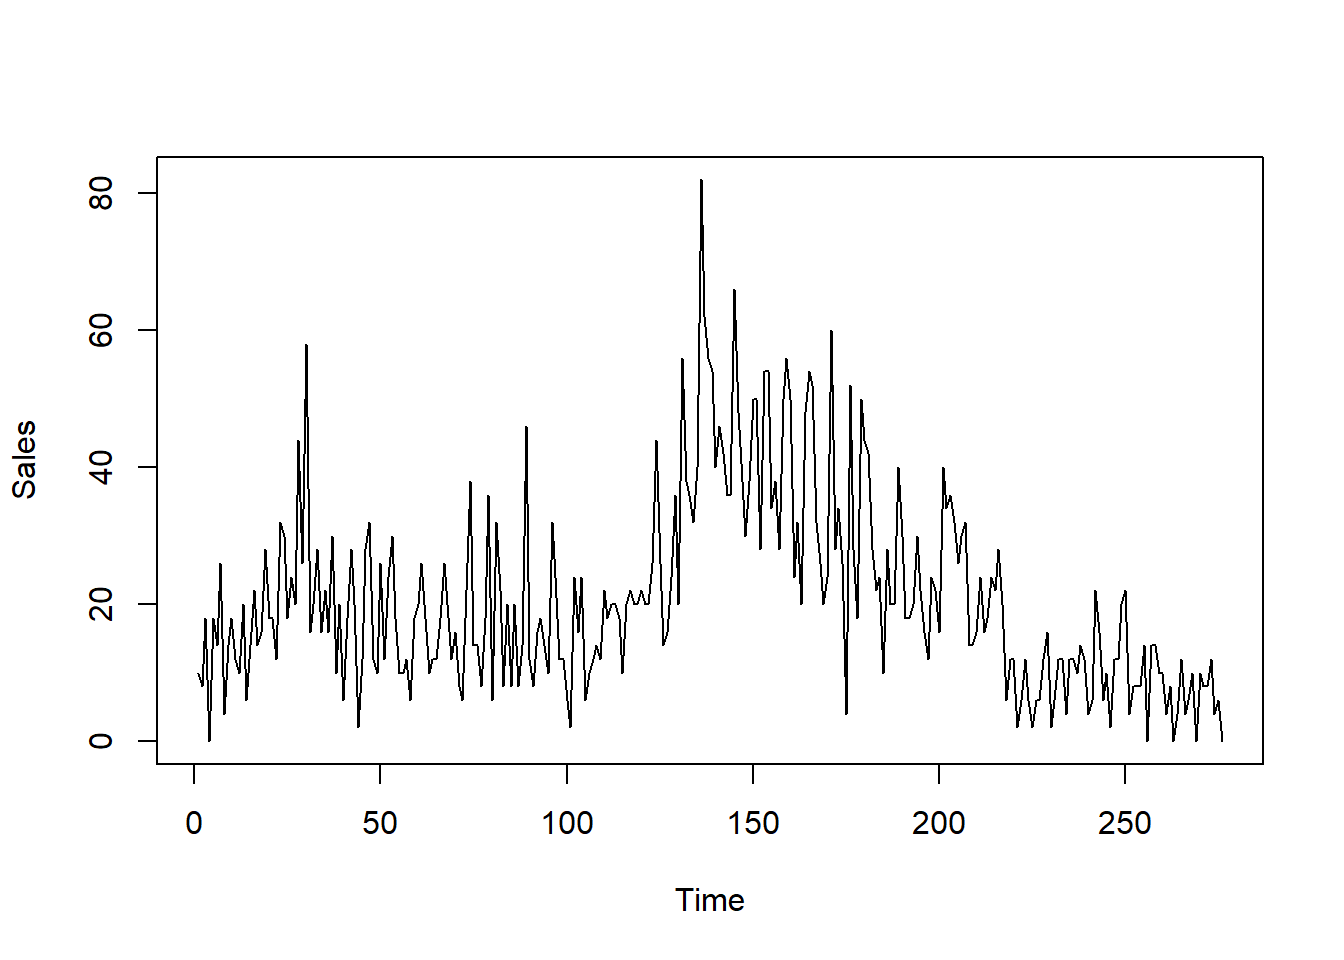
\includegraphics[scale=0.8]{FreshTS.png}
        \caption{生鲜日销量序列}
    \end{figure}
    如图所示,序列有比较明显的先上升再下降的趋势,因此采用以下3种模型拟合数据:
    \begin{itemize}
        \item ARIMA模型:建立ARIMA模型需要假设时间序列数据差分平稳,同时不能为白噪声数据,否则没有分析价值。
        模型表示为$x_t-x_{t-1}=\varepsilon_t-\theta\varepsilon_{t-1}$,其中$\varepsilon_t\sim N(0,\sigma_1^2)$。
        \item 残差自回归模型:因为数据有明显的先升后降趋势,可以先通过确定性因素分解方法提取序列中主要的确定性信息,假设残差项之间具有自相关关系,并拟合残差自回归模型提取。
        模型表示为$x_t=c+bt+at^2+\varepsilon_t$,$\varepsilon_t=\theta_1\varepsilon_{t-1}+\theta_5\varepsilon_{t-5}+e_t$,其中$e_t\sim N(0,\sigma_2^2)$。
        \item 线性回归模型:建立线性回归模型需要假设残差项满足Gauss假定。
        模型表示为$x_t=a_0+a_1t+a_2t^2+a_3t^3+a_4t^4+a_5t^5+\varepsilon_t$,其中$\varepsilon_t\sim N(0,\sigma_3^2)$。
    \end{itemize}
    \subsubsection*{B}
    利用训练集数据拟合模型,得到3个模型的参数,则拟合模型分别为:
    \begin{itemize}
        \item ARIMA(0,1,1):$x_t-x_{t-1}=\varepsilon_t+0.7998\varepsilon_{t-1}$,其中$\varepsilon_t\sim N(0,103.6)$。
        \item 残差自回归模型:$x_t=7.5760+0.3261t-0.001242t^2+\varepsilon_t$,$\varepsilon_t=0.3570\varepsilon_{t-1}+0.3358\varepsilon_{t-5}+e_t$,其中$e_t\sim N(0,101)$。
        \item 线性回归模型:$x_t=11.30+0.7897t-0.02476t^2+0.0002935t^3-0.000001363t^4+0.000000002131t^5+\varepsilon_t$,其中$\varepsilon_t\sim N(0,116.4241)$。
    \end{itemize}
    \subsubsection*{C}
    经检验,拟合模型显著,且模型参数显著。
\end{document}